\documentclass{standalone}
\usepackage{amsmath}
\usepackage{multicol}
\usepackage{tikz}
\usepackage{multirow}
\usepackage[lm]{sfmath} % For serif math

\usetikzlibrary{arrows}
\usetikzlibrary{calc}
\usetikzlibrary{decorations.pathreplacing}
\usetikzlibrary{positioning}

\tikzset{>=latex}

\renewcommand*\familydefault{\sfdefault}

\begin{document}

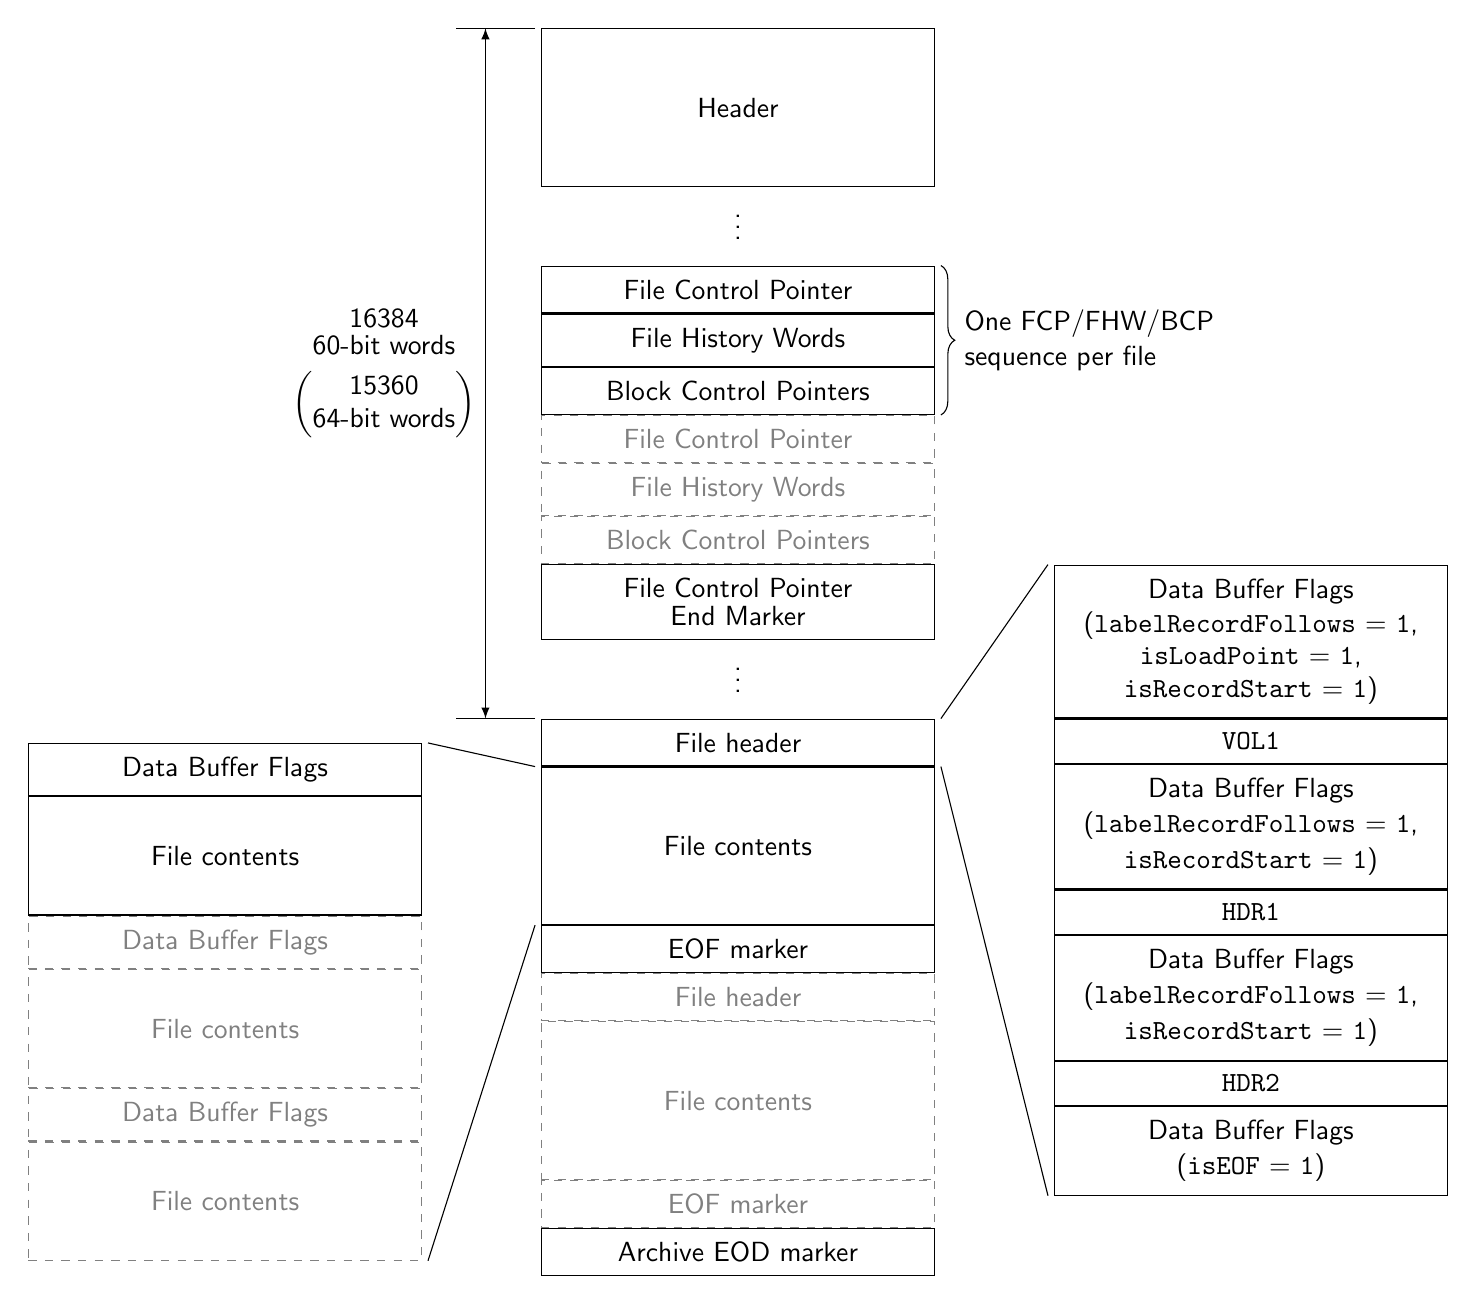
\begin{tikzpicture}[block/.style={draw,rectangle,inner sep=0.5em,minimum width=5cm}]

\node (header) [block,minimum height=2cm] {Header};
\node [block,below=of header] (fcp1) {File Control Pointer};
\node [block,below=0cm of fcp1] (fhw1) {File History Words};
\node [block,below=0cm of fhw1] (bcp1) {Block Control Pointers};
\node [block,dashed,gray,below=0cm of bcp1] (fcp2) {File Control Pointer};
\node [block,dashed,gray,below=0cm of fcp2] (fhw2) {File History Words};
\node [block,dashed,gray,below=0cm of fhw2] (bcp2) {Block Control Pointers};
\node [block,below=0cm of bcp2] (fcpend) {\shortstack[c]{File Control Pointer\\ End Marker}};
\node (filehead1) [block,below=of fcpend] {File header};
\node (contents1) [block,below=0cm of filehead1, minimum height=2cm] {File contents};
\node (eof1) [block,below=0cm of contents1] {EOF marker};
\node (filehead2) [block,gray,dashed,below=0cm of eof1] {File header};
\node (contents2) [block,gray,dashed,below=0cm of filehead2, minimum height=2cm] {File contents};
\node (eof2) [block,gray,dashed,below=0cm of contents2] {EOF marker};
\node (eod) [block,below=0cm of eof2] {Archive EOD marker};

\node at ($(header.south)!0.5!(fcp1.north)$) [yshift=2.5pt] {\vdots};
\node at ($(fcpend.south)!0.5!(filehead1.north)$) [yshift=2.5pt] {\vdots};

\draw [<->] ($(header.north west)+(left:0.7cm)$) --
            ($(filehead1.north west)+(left:0.7cm)$)
      node [midway,anchor=east] {\shortstack[c]{
          \shortstack[c]{16384\\60-bit words\\\phantom{}}\\
          \(\left(\begin{array}{@{}c@{}}\text{15360}\\\text{64-bit words}\end{array}\right)\)
      }};
\foreach \x in {header, filehead1} \draw ($(\x.north west)+(left:2pt)$) -- ++(left: 1.0cm);

\draw [decorate,decoration={brace,amplitude=5pt}]
      ($(fcp1.north east)+(right:2pt)$) -- ($(bcp1.south east)+(right:2pt)$)
      node [midway,anchor=west,xshift=0.5em] {\shortstack[l]{One FCP/FHW/BCP\\sequence per file}};

\node (FileHeadDBF1) [block,right=1.5cm of filehead1.north east,anchor=south west] {\shortstack[c]{Data Buffer Flags\\ (\texttt{labelRecordFollows} = \texttt{1},\\ \texttt{isLoadPoint} = \texttt{1},\\ \texttt{isRecordStart} = \texttt{1})}};
\node (FileHeadVOL1) [block,below=0cm of FileHeadDBF1] {\texttt{VOL1}};
\node (FileHeadDBF2) [block,below=0cm of FileHeadVOL1] {\shortstack[c]{Data Buffer Flags\\ (\texttt{labelRecordFollows} = \texttt{1},\\ \texttt{isRecordStart} = \texttt{1})}};
\node (FileHeadHDR1) [block,below=0cm of FileHeadDBF2] {\texttt{HDR1}};
\node (FileHeadDBF3) [block,below=0cm of FileHeadHDR1] {\shortstack[c]{Data Buffer Flags\\ (\texttt{labelRecordFollows} = \texttt{1},\\ \texttt{isRecordStart} = \texttt{1})}};
\node (FileHeadHDR2) [block,below=0cm of FileHeadDBF3] {\texttt{HDR2}};
\node (FileHeadDBF3) [block,below=0cm of FileHeadHDR2] {\shortstack[c]{Data Buffer Flags\\ (\texttt{isEOF} = \texttt{1})}};

\draw ($(filehead1.north east)+(right:2pt)$) -- ($(FileHeadDBF1.north west)+(left:2pt)$);
\draw ($(filehead1.south east)+(right:2pt)$) -- ($(FileHeadDBF3.south west)+(left:2pt)$);

\node (FileContentsDBF1) [block,left=1.5cm of contents1.north west,anchor=north east,yshift=0.3cm] {Data Buffer Flags};
\node (FileContentsChunk1) [block,below=0cm of FileContentsDBF1, minimum height=1.5cm] {File contents};
\node (FileContentsDBF2) [block,gray,dashed,below=0cm of FileContentsChunk1] {Data Buffer Flags};
\node (FileContentsChunk2) [block,gray,dashed,below=0cm of FileContentsDBF2, minimum height=1.5cm] {File contents};
\node (FileContentsDBF3) [block,gray,dashed,below=0cm of FileContentsChunk2] {Data Buffer Flags};
\node (FileContentsChunk3) [block,gray,dashed,below=0cm of FileContentsDBF3, minimum height=1.5cm] {File contents};

\draw ($(contents1.north west)+(left:2pt)$) -- ($(FileContentsDBF1.north east)+(right:2pt)$);
\draw ($(contents1.south west)+(left:2pt)$) -- ($(FileContentsChunk3.south east)+(right:2pt)$);

\end{tikzpicture}

\end{document}
